\section{Test}
Testing er en grundsten i ethvert succesfuldt softwaresystem. Uden testing kan
der ikke stilles garanti for et systems opførsel. Nedenstående afsnit dækker
alle test foretaget af "Dungeons and Gnoblins" spillet, for at sikre den korrekte
opførsel i henhold til kravspecifikationerne.

Her dækkes test af alle de største komponenter, Frontend, Game Engine, Backend og
database. Testene inkluderer automatiseret unittests, integrationstest og accepttest.

\subsection{Modultest Frontend}
Modultesten af Frontenden er lavet i meget tæt samarbejde med Game Engine holdet. Dette er valgt sådan, at når Game Engine lavede en ny funktion eller funktionalitet, gik frontend holdet igang med at implementere en visuel repræsentation af denne nye funktion/funktionalitet. Således var det ikke kun en visuel test af at views så godt ud eller at man kunne trykke på en knap, men derimod kunne både frontenden og Game Enginen testes i samarbejde, hvor den reelle funktionalitet for systemet blev testet.

\subsubsection{Test metoder}
Hver gang der er blevet lavet små eller større ændringer i frontenden, er der blevet lavet både en funktionel og visuel test af de nye ændringer. Dette blev gjort for æstetiske ændringer ved at kigge i preview vinduet i WPF for det view der blev ændret. Var det derimod en ændring der inkluderede databinding til Game Enginen, blev det nødvendigt at teste hele programmet ved brug af compileren og derved lave en runtest, som inkluderede at det rigtige data blev hentet fra Game Enginen eller at den rigtige funktionalitet blev kaldt ved et tryk på en knap.

\subsubsection{Eksempel på frontend test i forbindelse med Game Engine}
Et godt eksempel på hvordan frontend testene blev kørt er ved implementeringen af Room-viewets map element og mere specifikt bevægelsen fra et rum til et andet, altså de implementerede "Go North,East,South,West" knapper, som krævede både en visuel og funktionel del.\\
Den visuelle del bestod i at kortet skulle opdateres, spilleren flyttes og rum-beskrivelsen opdateres.\\
Den funktionelle del bestod i at Game Enginen skulle kontaktes på korrekt vis med rigtige parametre. De rigtige databindings skulle opdateres, således at den visuelle del blev opdateret korrekt og derefter skulle informationen om det rum gemmes korrekt i Game Enginen.\\
For at være sikker på at alt data blev opdateret korrekt blev programmet kørt i debug mode, hvor der kunne sættes break-points i koden og værdierne på diverse variabler, såsom roomdescription og currentroom kunne undersøges. Samtidig blev der kigget på den visuelle del af selve viewet, hvor der blev tjekket om beskrivelsen blev korrekt displayet, mappen opdateret korrekt og at spilleren flyttes korrekt.
\subsubsection{Eksempel på frontend test}
Ikke alle moduler krævede at Game Enginen blev kontaktet. Eksempelvis Mediatoren, som er beskrevet i Frontend implementings afsnittet som kan findes her: \autoref{sec:Frontend Implementering}. Med dette modul blev der lavet mocks, hvor vi satte en dummy knap op til at kunne kalde notify() funktionen i Mediatoren og der blev tjekket visuelt om viewet blev skiftet uden at hele applikationsvinduet blev skiftet og at det korrekte view blev vist. 
\subsection{Modultest Game Engine}
Game Engine styrer spillets indre logik. Dette dækker over alt fra spillerens bevægelse gennem spillet til "save" og "load" af nye og gamle spil.
Det er derfor yderst nødvendigt at denne er fuld testet.

For at sikre Høj kvalitet er Game Engine skrevet med Robert C. Martins
``Three Laws of TDD'' \parencite{CleanCode} i baghoved hvilket medfører til at Game Engine er 
eksklusivt test ved hjælp af black-box testing. Alle testene tester
kun det offentlige interface, som er gjort tilgængelig. 
\newpage 

\subsubsection{GodkendelsesTabel Game Engine}
Nedestående præsenteres en fuld tabel for alle classes testet som 
led i Game Engine. De vigtigste er GameController, CombatController,
Player/Room og DiceRoller. Dice danner ``Core Mechanics'' for spillet.

Interessant nok ses her at GameController fejler sine test grundet at
der ikke er skrevet test til mange af GameControllerens ansvars punkter.

\begin{center}
\captionof{table}{Her Ses en komplet liste over alle test foretages på
                  Game Engine komponenter, med kommentar til deres resultater
                  og en endelig vurdering af test resultaterne.}
\vspace{-1em}
\label{tab:testEngine}
  \begin{longtable}{|l|p{0.25\linewidth}|p{0.25\linewidth}|l|}
  \hline
  \multicolumn{4}{|c|}{\textbf{Game Engine GodkendelsesTabel}} \\ \hline
  \textbf{Komponent under test} & \textbf{Forventet Adfærd} & \textbf{Kommentar} & \textbf{Test Resultat} \\ \hline
  Game Controller
  &
    \begin{enumerate}
      \item \begin{flushleft} Kan skifte Player til Nyt Room \end{flushleft}
      \item \begin{flushleft} Kan samle Item op fra Room  \end{flushleft}
      \item \begin{flushleft} Kan save Game \end{flushleft}
      \item \begin{flushleft} Kan loaded Games \end{flushleft}
      \item \begin{flushleft} Kan eliminere Enemy fra Game \end{flushleft}
      \item \begin{flushleft} Kan reset Game \end{flushleft}
      \item \begin{flushleft} Kan anskaffe Room description \end{flushleft}
    \end{enumerate}
  &
  \flushleft 
  Game Controller er kun test for at skifte til nyt Room, dette betyder at der 
  ikke kan stilles garanti for at resterende implementeringer af load- og save game
  osv. fungere som ønsket. Disse ting er svagt testet gennem visuelt trial and error
  test, men da der ikke er skrevet nogen specifikke test til dem Fejler 
  GameControlleren sin komponent test.
  &
  FAIL
  \\ \hline
  Combat Controller
  &
  \begin{enumerate}
    \item \begin{flushleft} Kan Håndtere Combat Rounds \end{flushleft}
    \item \begin{flushleft} Kan håndtere at Player løber væk fra Combat \end{flushleft}
  \end{enumerate}
  &
  \flushleft
  Combat controller kan håndtere at spilleren løber fra combat og at Player indgår i combat.
  CombatController kan stille garanti for at combat sker i den rigtige orden og at hverken
  spiller eller enemy kan angribe hvis denne er død.
  Ydmere stiller den garanti for at både enemy og spiller kan lave ``critial hits'' hvis dice
  rolleren slår 20.
  &
  OK
  \\ \hline
  DiceRoller
  &
  \begin{enumerate}
    \item \begin{flushleft} Kan emulerer et kast med en N siddet terning \end{flushleft}
    \item \begin{flushleft} Kan emulerer N kast med en M siddet terning \end{flushleft}
  \end{enumerate}
  &
  \flushleft
  DiceRoller Kan emulere et eller flere terninge kast med samme antal sidder. Denne kan
  ydmere stille krav for at fordellingen af disse terningekast har en normal distribution 
  og dermed er alle udfald lige sandsynlige.
  &
  OK
  \\ \hline
  BaseMapCreator
  &
  \begin{enumerate}
    \item \begin{flushleft} Kan generere et map layout file \end{flushleft}
  \end{enumerate}
  &
  \flushleft
  BaseMapCreator can på korrekt vis generere et map layout file, den kan ydmere
  generer item layout files og Enemy layout files, der hjælper Map klassen med 
  at genererer spillet Map. Der ikke skrevet test for eksistensen af item og enemy 
  layout Map og derfor kan der ikke stille garanti for at disse bliver genereret 
  på korrektvis. Testen Fejler derfor.
  &
  FAIL
  \\ \hline
  BaseMap
  &
  \begin{enumerate}
    \item \begin{flushleft} Kan anskaffe Rooms ud fra en Direction \end{flushleft}
  \end{enumerate}
  &
  \flushleft
  Map kan anskaffe Rooms uf fra en given Direction. Map kan på korrektvis generer et 
  map udfra mappets layout file. Den kan også på korrektvis finde udaf hvilke Rooms
  har adgang til hinanden. Der er ikke skrevet test for at bekræfte at enemy og items er 
  i de korrekte lokationer baseret på enemy og item layout filerne.
  Derfor fejler denne sin Test.
  &
  FAIL
  \\ \hline
  Player
  &
  \begin{enumerate}
    \item \begin{flushleft} Kan angribe Enemy  \end{flushleft}
    \item \begin{flushleft} Kan tage skade \end{flushleft}
    \item \begin{flushleft} Kan skade Enemy (Ikke Kristisk)  \end{flushleft}
    \item \begin{flushleft} Kan skade Enemy (Kritisk)  \end{flushleft}
  \end{enumerate}
  &
  \flushleft
  Player kan angribe, skade og tage skade fra enemy. 
  &
  OK
  \\ \hline
  Enemy
  &
  \begin{enumerate}
    \item \begin{flushleft} Kan angribe Player  \end{flushleft}
    \item \begin{flushleft} Kan tage skade \end{flushleft}
    \item \begin{flushleft} Kan skade Player (Ikke Kristisk)  \end{flushleft}
    \item \begin{flushleft} Kan skade Player (Kritisk)  \end{flushleft}
  \end{enumerate}
  &
  \flushleft
  Enemy kan angribe, skade og tage skade fra Player.
  &
  OK
  \\ \hline
  Log
  &
  \begin{enumerate}
    \item \begin{flushleft} Kan log et event \end{flushleft}
    \item \begin{flushleft} Kan anskaffe et event \end{flushleft}
    \item \begin{flushleft} Kan merge to logs \end{flushleft}
  \end{enumerate}
  &
  \flushleft
  Log kan logge et event, anskaffe eventet og merge to forskellige logs.
  &
  OK
  \\ \hline
  Room                          
  & 
  \begin{enumerate}
    \item Kan tilføje Player
    \item Kan tilføje Enemy
    \item Kan fjerne Player
    \item kan fjerne Enemy
  \end{enumerate}
  &
  \flushleft
  Room kan fjerne/tilføje Player og Enemy som forventet
  &
  OK
  \\ \hline
  Items
  &
  \begin{enumerate}
    \item[]
  \end{enumerate}
  &
  \flushleft
  Items så som sword, shield, axe osv.\ indeholder kun data og har derfor ikke nogen
  testbar adfærd andet end deres constructor. De kan alle construeres på korrekt vis.
  &
  OK
  \\ \hline
\end{longtable}
\addtocounter{table}{-1}
\end{center}

\newpage 

\subsubsection{Mock testing}
I nogle tilfælde kan det være umuligt er lave troværdige tests, når
en klasse f.eks. Player er dyb afhængig af DiceRoller klassen. Dette skyldes
at DiceRoller danner pseudo-random outputs og derfor er test med den ikke 
altid troværdige.

Her benyttes mock tests og dependency injections til at sikre at DiceRoller 
klassen danner de samme outputs hver gang en test køres.
Derved kan alle senarier for Player klassen testes, hvor man kan regne med at DiceRoller giver et bestemt output. 

\begin{figure}[H]
  \centering
  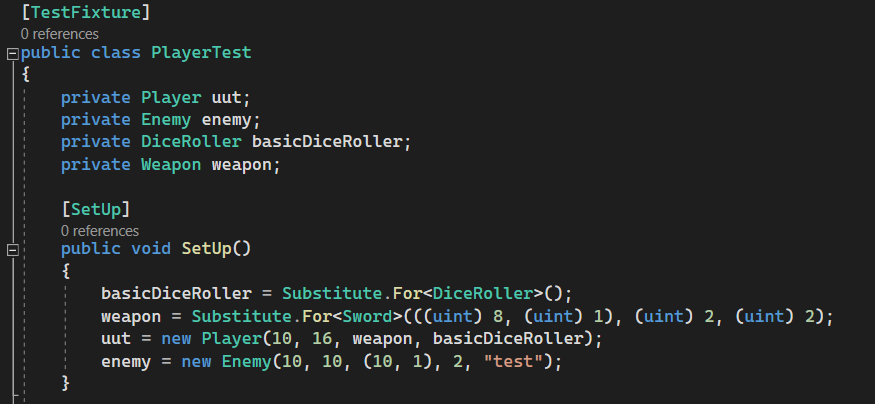
\includegraphics[scale=0.5]{02-Body/Images/Mocks_And_Dependency_Injection.png}
    \caption{}
  \label{fig:mock}
\end{figure}

\begin{figure}[H]
  \centering
  \includegraphics[scale=0.45]{02-body/Images/useofmocks.png}
    \caption{Mocks benyttes her til at sikre at dependencien, her DiceRoller, returner
           den ønskede værdi for situationen, der er under test.
           Alle test tildeles informative navne, for at sikre læsbarhed i forhold 
           til testenes formål.}
  \label{fig:mockuse}
\end{figure}

\newpage 

\subsubsection{Test Resultater for Game Engine}
Nedestående vises kort resultatet for Game Engine test, når de alle køres via visual studio. Som det kan ses så er alle testene succesfulde, hvilket giver hvis garanti for at
game engine opfører sig som specificeret i kravspecifikationerne og i de implementerede interfaces.

\begin{figure}[H]
  \centering
  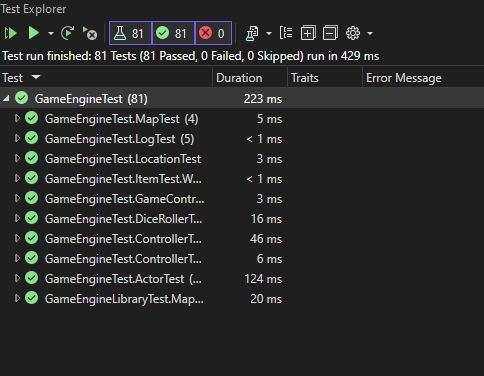
\includegraphics[scale=0.4]{02-body/Images/Test Results.png}
    \caption{Alle skrevene test til Game Engine passer, hvilket hjælper med at give vished
          om at Game Engine udfører dens funktionalitet, som det er beskrevet i kravene.
          Dette siges da alle testene er skrevet på baggrund af kravene som black-box tests
          og ikke som white-box test efter implementeringen.}
  \label{fig:TestResultsGameEngine}
\end{figure}





\newpage

\input{02-Body/Test/Database-Modultest.tex}
\subsection{Backend Modultest}

Dette afsnit omhandler modultesten af backenden, denne deles op i følgende to dele, der fortages først en modultest af DAL som kan findes her \autoref{ssec: Modultest database} , hvorefter DAL bruges i modultesten af Web api’et, da Web api’et ikke vil blive testet uden DAL modulet.\\

Til at udføre modultests af web api’et benyttes udviklingsværktøjet Swashbuckle \cite{Swagger}. Swashbuckle bruges til at bygge SwaggerDocument objekter på baggrund af de routes, controllers og modeller som er blevet udviklet. Hertil tilbyder Swashbuckle et Swagger User interface, hvor man kan teste sine http funktioner og se om man modtager den forventede response. Derfor er dette et oplagt værktøj at gøre brug af. Et billede af Swagger User interfacet kan ses på \autoref{fig:Modultest-Backend-swagger}.\\

\begin{figure}[H]
\centering
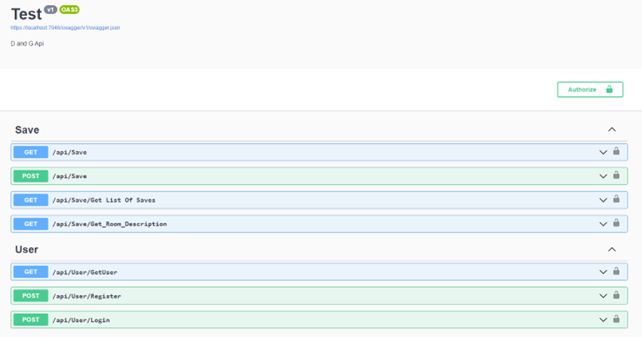
\includegraphics[width = \textwidth]{02-Body/Images/Backend_swagger.PNG}
\caption{Swagger User interface, som viser de forskellige http metoder}
\label{fig:Modultest-Backend-swagger}
\end{figure}

For at aktivere swagger tilføjes følgende middleware til program.cs AddSwaggerGen(), UseSwagger() og UseSwaggerUI(). Til SwaggerGen tilføjes også security med JWT tokens så Authentication og Authorization kan testes.\\

I \autoref{table: succes} kan ses en tabel oversigt over tests af succes scenarie, for de enkelte funktioner samt resultater.\\


\begin{table}[H]
\label{table: succes}
\caption{Tabel over modultest af Backendes Web Api, her vises testes af succes scenarier for alle Web Api http funktioner }%
\begin{tabular}{|p{0.75cm}|p{3.6cm}|p{3.5cm}|p{3.5cm}|p{1.9cm}|} \hline
 \textbf{Test} & \textbf{Funktion} & \textbf{Forventet resultat} & \textbf{Observering} & \textbf{Vurdering} \textbf{(OK/Fail)}\\\hline
 1 & PostSave(SaveDTO saveDTO) & Der bliver sendt et specifikt gamestate, for brugeren der er logget ind. & Det er muligt at sende game statet, og de korrekte værdier bliver sendt med. & OK \\ \hline
 2 & Register(UserDTO regUser) & Der registreres en ny bruger, ved at gemme oplysninger omkring denne. Der returneres en JWT-token. & Brugeren bliver registreret, og kan findes blandt de andre brugere. Det ses at der returneres en JWT-token. & OK \\ \hline
 3 & Login(UserDTO userDTO) & Der tjekkes om oplysningerne passer med en registreret bruger, og passer det logges der ind. Der returneres en JWT-token. & Det lykkedes at logge ind, og der returneres en JWT-token.  & OK \\ \hline
 4 & GetSave(int id) & Der hentes et specifikt save for den bruger der er logget ind. & Det lykkedes at hente et specifikt game state, uden errors  & OK \\ \hline
 5 & GetListOfSave() & Der hentes en liste af game states, for brugeren der er logget ind. & Det lykkedes at hente en liste af game states, for den specifikke bruger. & OK \\ \hline
 6 & GetRoomDescription(int id) & Denne route henter en beskrivelse af det valgt rum i spillet. & Det ses, at der bliver hentet en beskrivelse af det valgte rum. & OK \\ \hline
\end{tabular}
\end{table}

I nesdstående tabel \label{table: fejl} testes om funktionerne håndtere fejlscenarier korrekt.

\begin{table}[H]
\label{table: fejl}
\caption{Tabel over modultest af Backendes Web Api, her vises testes af fejlscenarier for alle Web Api http funktioner}%
\begin{tabular}{|p{0.75cm}|p{3.6cm}|p{3.5cm}|p{3.5cm}|p{1.9cm}|} \hline
 \textbf{Test} & \textbf{Funktion} & \textbf{Forventet resultat} & \textbf{Observering} & \textbf{Vurdering} \textbf{(OK/Fail)}\\\hline
 1 & Register(UserDTO regUser) & Brugernavnet er allerede i brug, og der sendes en fejlmeddelelse  & Status: 400. Besked: ”Name is already in use”. & OK \\ \hline
 2 & Login(UserDTO userDTO) & Oplysningerne stemmer ikke overens med en registreret bruger, og der bør sendes en fejlmeddelelse. & Status: 400. Besked: ”Wrong Username or Password” & OK \\ \hline
 3 & GetSave(int id) & Der er ikke logget ind, så der kan ikke hentes et game state. & Status: 401, Unauthorized & OK \\ \hline
 4 & GetListOfSave() & Der er ikke logget ind, og derfor kan der ikke hentes et liste. &Status: 401, Unauthorized  & OK \\ \hline
 5 & PostSave(SaveDTO saveDTO) & Der er ikke logget ind, og derfor kan der ikke gemmes er spil. & Status: 401, Unauthorized & OK \\ \hline

\end{tabular}
\end{table}

Med alle funktioner testet med et godkent resultat, er backenden klar til at blive integreret med de andre moduler for systemet.



\newpage

\section{Integrationstest}
\subsection{Tidlig Integrationstest}
For gruppen var det et mål at komme igang med at lave integrationstest så hurtigt som muligt, da vi ønskede at der hurtigt kom styr på kommunikationen mellem de forskellige moduler i systemet. Her integreres altså blot vores MVP se Tekniskbilag (sektion 3.1) og det ville derefter være nemmere at implementere nye features.\\

\noindent For at køre systemet har vi først startet den oprettede docker container til spillets database. Derefter startede vi spillets server, i form af en backend api. Til slut kunne spillets klient åbnes og systemet testes.\\

\noindent I den tidlige integrationstest løb vi som gruppe ind nogle forskellige problemer.\\
Vi havde som gruppe arbejdet for opdelt i forskellige dokumenter. 
Derudover opdagede vi at de forskellige projekter benyttede forskellige versioner af .net, dette var dog hurtigt løst.\\
Til slut opdagede vi at der, når man loader et spil, ikke blev vist for brugeren hvilken rum man havde besøgt. Dette blev diskuteret og gruppen besluttede at tilføje dette til næste iterationer.\\

\noindent I det vedhæftede MVP Video bilag ses en demonstrations video af integrationstesten af MVP. Her det ses at man kan spille spillet, gemme det og derefter loade det korrekt ind igen, dog igen uden at man kan se hvilke rum man har besøgt.


\subsection{Fulde Integrationstest}

Med den indledende integrationstest, er kommunikationen igennem sytemet på plads, samt de basale funktionaliteter. Herfeter udvides spillet med flere features som: Login, Register, Enemies, Items, Health, EquipedItems, Shield, Combat, Map Visibility og Room Descriptions. Dette er features, som kræver yderligere udvikling indenfor alle tekniske områder af projektet.\\

\noindent Feature udviklingen i Frontend og Game Engine Modul udvikles sammen, derfor er de moduler allerede integreret med hinanden, det samme gælder for Backend og Databasen.\\

\noindent Der laves endnu en integrations test med alle de nye features. Her opstod en række nye problemer hvad angår Http kommuniaktionen imellem backend'en og frontend'en. Dette bundede i overenstemmelsen af data modellerne på backend og frontend siden. Det drejede sig helt specifikt omkring de nyeligt tilføjede properties til modellen "Save", på fronted'en blev brugt datatypen uint imens der på backend blev brugt int, samtidigt med at properties hed noget forskelligt. Derfor blev de nye properties ignorede når data'en blev seraliseret og deseraliseret. Dette problem var ikke noget som debuggeren gjorde opmærksom på derfor tog det relativt lang tid at få det løst.\\

\noindent Et andet problem som opstod, var angående Room Description, her blev det besluttet under implementering at gemme dem i databasen fremfor lokalt, grundet problemer med resources og deres specifikke stier på forskellige pc'er.\\

\noindent Med disse problemer løst, resulterede integrationstesten i vores færdige produkt, som blev anvendt i acceptesten. Acceptesten samt en demonstrations video af produktet kan ses her. \textbf{REF TIL VIDEO AF ACCEPTEST VIDEO}    
 

  


\section{Accepttestspecifikation}
For accepttestspecifikationen er der opstillet tests for dette projekt, og på baggrund af disse kan det betragtes som et funktionelt og acceptabelt produkt. Denne accepttestspecifikation er delt op i Funktionelle krav og ikke funktionelle krav.

\subsection{Funktionelle}
\paragraph{Test af User Story 1 - Login}

\textbf{Scenarie - Succesfuld login}

\textit{Givet at brugerens profil er oprettet på databasen og at serveren er oppe.}

\begin{itemize}
  \item Når bruger indtaster sit login(Brugernavn og password)
  \item og trykker "Log in" på UI
  \item Så skifter skærmen til hovedmenu
\end{itemize}

Resultat: Godkendt\\
Kommentar:\\

\textbf{Scenarie - Fejlet login}

\textit{Givet at brugerens profil er oprettet på databasen og at serveren er oppe.}

\begin{itemize}
  \item Når bruger indtaster et forkert login(Brugernavn og password)
  \item og trykker "Log in" på UI
  \item Så signaleres der om forkert login-oplysninger til bruger
\end{itemize}

Resultat: Godkendt\\
Kommentar: Viser korrekt error besked\\

\paragraph{Test af User Story 2 - Opret profil}

\textbf{Scenarie - Bruger opretter profil}

\textit{Givet at brugerens profil er oprettet på databasen og at serveren er oppe.}

\begin{itemize}
  \item Når bruger vælger at oprette profil
  \item Så gemmes datanene for brugerens profil på databasen
  \item Og skærmen skiftes til log ind skærmen
\end{itemize}

Resultat: Godkendt\\
Kommentar:\\

\textbf{Scenarie - Bruger opretter samme profil}

\textit{Givet at brugerens profil er oprettet på databasen og at serveren er oppe.}

\begin{itemize}
  \item Når bruger vælger at oprette en allerede-eksisterende profil
  \item Så signaleres der om at profil allerede eksisterer
\end{itemize}

Resultat: Godkendt\\
Kommentar: Viser korrekt error besked\\

\paragraph{Test af User Story 3 og 4 - Main Menu}

\textbf{Scenarie - Tilgå settings}

\textit{Givet at brugeren er logget ind og har adgang til spillet.}

\begin{itemize}
  \item Når bruger trykker settings i UI
  \item Så går spillet til settings menuen
\end{itemize}

Resultat: Godkendt\\
Kommentar:\\

\textbf{Scenarie - Start spillet}

\textit{Givet at brugeren er logget ind og har adgang til spillet.}

\begin{itemize}
  \item Når bruger trykker "New Game"
  \item Så vises game-interface for brugeren
\end{itemize}

Resultat: Godkendt\\
Kommentar:\\

\textbf{Scenarie - Exit game}

\textit{Givet at brugeren er logget ind og har adgang til spillet.}

\begin{itemize}
  \item Når bruger trykker "Exit game"
  \item Så lukker spillet
\end{itemize}

Resultat: Godkendt\\
Kommentar:\\

\paragraph{Test af User Story 5-16 - Exit Menu}

\textbf{Scenarie - Exit spil}

\textit{Givet at brugeren har trykket "New Game"}

\begin{itemize}
  \item Når bruger trykker "Escape" på keyboardet
  \item Så popper et menuvindue op med mulighederne "Resume Game", "Save Game", ”Main Menu" og "Settings"
\end{itemize}

Resultat: Godkendt\\
Kommentar:\\

\textbf{Scenarie - In game menu - Resume game}

\textit{Givet at brugeren har trykket "New Game" og derefter har trykket "Escape" på keyboard}

\begin{itemize}
  \item Når bruger trykker "Resume Game" i In game menu
  \item Så forsvinder menuvinduet og spillet fortsætter
\end{itemize}

Resultat: Godkendt\\
Kommentar:\\

\textbf{Scenarie - In game menu - Save -- No Combat}

\textit{Givet at brugeren har trykket "New Game" og derefter har trykket "Escape" på keyboard}

\begin{itemize}
  \item Når bruger trykker på "Save Game" i In game menuen
  \item Så vises save menuen
  \item Og en liste af gemte spil
\end{itemize}

Resultat: Godkendt\\
Kommentar: Der vises maks. fem spil\\

\textbf{Scenarie - In game menu - Save -- Combat}

\textit{Givet at brugeren er i combat}

\begin{itemize}
  \item Når bruger trykker "Escape" på keyboarded
  \item Så kan man ikke se en "Save Game" knap i game menuen
\end{itemize}

Resultat: Godkendt\\
Kommentar:\\

\textbf{Scenarie - In game menu - Main Menu}

\textit{Givet at brugeren har trykket "New Game" og derefter har trykket "Escape" på keyboard}

\begin{itemize}
  \item Når bruger trykker "Main Menu" i In game menu
  \item Så vises hovedmenuen
\end{itemize}

Resultat: Godkendt\\
Kommentar:\\

\textbf{Scenarie - In game menu - Settings}

\textit{Givet at brugeren har trykket "New Game" og derefter har trykket "Escape" på keyboard}

\begin{itemize}
  \item Når bruger trykker "Settings"
  \item Så åbnes et vindue med mulighed for konfiguration af spil for bruger
\end{itemize}

Resultat: Godkendt\\
Kommentar:\\

\textbf{Scenarie - Exit menu - Settings - Apply}

\textit{Givet at brugeren har trykket "Settings" og ændret på resolution indstilling}

\begin{itemize}
  \item Når bruger trykker "Apply"
  \item Så ændres indstillinger som brugeren har ændret
\end{itemize}

Resultat: Godkendt\\
Kommentar: Skærm opløsning ændres korrekt\\

\textbf{Scenarie - Exit menu - Settings - Back}

\textit{Givet at brugeren har trykket "Settings"}

\begin{itemize}
  \item Når bruger trykker "Back"
  \item Så vises In game menuen
\end{itemize}

Resultat: Godkendt\\
Kommentar:\\

\textbf{Scenarie - Exit menu - Settings - Default}

\textit{Givet at brugeren har trykket "Settings" og har ændret mindst 1 indstlling}

\begin{itemize}
  \item Når bruger trykker "Default"
  \item Så ændres alle indstiliinger tilbage til default settings
\end{itemize}

Resultat: Godkendt\\
Kommentar: Indstillinger ændres til Default indstillinger korrekt.\\

\paragraph{Test af User Story 17 og 18 - Save Menu}

\textbf{Scenarie - Save Menu - Save Game}

\textit{Givet at brugeren har trykket "Save game" fra Settings menu og ikke er i combat.}

\begin{itemize}
  \item Når bruger vælger et gemt spil
  \item Og sætter navnet til det ønskede
  \item Og trykker på "Save Game" knappen
  \item Så genoptages spillet
\end{itemize}

Resultat: Godkendt\\
Kommentar:\\

\textbf{Scenarie - Save Menu - Back}

\textit{Givet at brugeren har trykket "Save game" fra Settings menu}

\begin{itemize}
  \item Når bruger trykker "Back" i save game menuen
  \item Så vender spillet ilbage til In game menuen
\end{itemize}

Resultat: Godkendt\\
Kommentar:\\

\paragraph{Test af User Story 19-22 - Main Menu}

\textbf{Scenarie - Main menu - Load Game}

\textit{Givet at brugeren er logget ind og har adgang til spillet.}

\begin{itemize}
  \item Når bruger trykker "Load game"
  \item Så vises en liste af gemte spil på profilen
\end{itemize}

Resultat: Godkendt\\
Kommentar:\\

\textbf{Scenarie - Main menu - Load Game - Load}

\textit{Givet at brugeren er logget ind og har adgang til spillet og trykket "Load Game"}

\begin{itemize}
  \item Når bruger vælger et gemt spil
  \item Og trykker "Load Game"
  \item Så loader spillet det gemte spil med det valgte game state
\end{itemize}

Resultat: Godkendt\\
Kommentar: Bruger starter i korrekt rum med korrekt inventory\\

\textbf{Scenarie - Main menu - Load Game - Back}

\textit{Givet at brugeren er logget ind og har adgang til spillet og trykket "Load Game"}

\begin{itemize}
  \item Når bruger trykker "Back" i load game-menuen
  \item Så vender spillet tilbage til hovedmenuen
\end{itemize}

Resultat: Godkendt\\
Kommentar:\\

\paragraph{Test af User Story 23-28 - Spil spillet}

\textbf{Scenarie - Spil spillet - Start spillet}

\textit{Givet at brugeren har trykket "New Game"}

\begin{itemize}
  \item Når bruger anvender piltasterne på keyboard eller trykker på knappen på interfacet til at bevæge sig sydpå fra startrummet
  \item Så bevæger brugeren sig ind i rummet "Syd" for det rum de står i
\end{itemize}

Resultat: Godkendt\\
Kommentar:\\

\textbf{Scenarie - Spil spillet - Enter nyt room}

\textit{Givet at brugeren har trykket "New Game"}

\begin{itemize}
  \item Når bruger går ind i et nyt rum ved brug af keyboard
  \item Så giver UI en beskrivelse af rummet spilleren befinder sig i
\end{itemize}

Resultat: Godkendt\\
Kommentar: Rum beskrivelser ændres korrekt når spiller går i nyt rum\\

\textbf{Scenarie - Spil spillet - Combat}

\textit{Givet at brugeren møder en fjende i et rum}

\begin{itemize}
  \item Når bruger trykker "Fight!"
  \item Så ruller brugeren et tal mod fjenden om at skade fjenden
  \item Og derefter ruller fjenden et tal om at skade brugeren
\end{itemize}

Resultat: Fejl\\
Kommentar: Kravet er testes af unit tests, så der vides at det er korrekt, men det kan ikke bekræftes visuelt\\

\textbf{Scenarie - Spil spillet - Combat - Flygt}

\textit{Givet at brugeren møder en fjende i et rum}

\begin{itemize}
  \item Når bruger trykker "Flee"
  \item Så flyttes brugeren tilbage til det rum han kom fra
  \item Og får ikke sit mistede liv tilbage igen
\end{itemize}

Resultat: Godkendt\\
Kommentar:\\

\textbf{Scenarie - Spil spillet - Inventory}

\textit{Givet at brugeren har trykket "New Game"}

\begin{itemize}
  \item Når bruger trykker "Inventory"
  \item Så vises genstande som bruger besidder
\end{itemize}

Resultat: Godkendt\\
Kommentar:\\

\textbf{Scenarie - Spil spillet - Interact}

\textit{Givet at brugeren har trykket "Start spil" og at der ike er fjender i rummet}

\begin{itemize}
  \item Når bruger trykker "Interact"
  \item Så kan bruger tage potentielle genstande i rummet til brugerens "Inventory"
\end{itemize}

Resultat: Godkendt\\
Kommentar:\\

\textbf{Scenarie - Spil spillet - Level klaret}

\textit{Givet at brugeren har fuldført det næstsidste rum}

\begin{itemize}
  \item Når bruger bevæger sig ind i sidste rum
  \item Så får bruger en besked om at spillet er klaret og får mulighed for at gå til "Main Menu"
\end{itemize}

Resultat: Fejl\\
Kommentar: Bruger kan gå til main menu, men sidste beskrivelse giver en uklar besked.\\

\subsection{ikke-funktionelle}
\textbf{GUI}
\begin{table}[H]
\caption{ Fuldført ikke funktionelle tests for GUI}
\label{tab:}
\begin{tabular}{|p{3cm}|p{3cm}|p{3cm}|p{3cm}|}
\hline
Beskrivelse & Verificering & Resultat & Kommentar \\
\hline
GUI'en skal tilbyde valget mellem 3 resolutions & Visuel & Godkendt & \\
\hline
GUI'en skal kunne være fullscreen & Visuel & Fejl & Window bar kunne ikke fjernes i fuldskærms opløsning\\
\hline
GUI'en skal kunne være windowed & Visuel & Godkendt & \\
\hline
\end{tabular}
\end{table}

\textbf{SOUND}
\begin{table}[H]
\caption{ Fuldført ikke funktionelle tests for SOUND}
\label{tab:}
\begin{tabular}{|p{3cm}|p{3cm}|p{3cm}|p{3cm}|}
\hline
Beskrivelse & Verificering & Resultat & Kommentar \\
\hline
Lyden skal kunne justeres mellem 0-100\% relativt til PC'ens lyd niveau. & Auditorisk/Visuel & Godkendt & \\
\hline
\end{tabular}
\end{table}

\textbf{DATABASE}
\begin{table}[H]
\caption{ Fuldført ikke funktionelle tests for DATABASE}
\label{tab:}
\begin{tabular}{|p{3cm}|p{3cm}|p{3cm}|p{3cm}|}
\hline
Beskrivelse & Verificering & Resultat & Kommentar \\
\hline
Skal kunne gemme maksimalt 5 save games & Visuel & Fejl & Back-end begrænser antal gemte spil, databasen kan indeholde flere gemte spil end fem.  \\
\hline
Skal kunne loade et spil indenfor maksimalt 5s & Visuel & Godkendt &\\
\hline
Skal gemme hvilke genstande man bruger lige nu & Visuel & Godkendt & \\
\hline
Skal gemme hvor meget liv man har tilbage. & Visuel & Godkendt & \\
\hline
Skal gemme hvilke fjender man har slået ihjel. & Visuel & Godkendt & \\
\hline
Skal gemme hvilke puzzles man har løst & Visuel & Fejl & Puzzles er ikke implementeret \\
\hline
Skal gemme hvilke rum man har været i. & Visuel & Godkendt & \\
\hline
\end{tabular}
\end{table}

\textbf{GAMEPLAY}
\begin{table}[H]
\caption{ Fuldført ikke funktionelle tests for GAMEPLAY}
\label{tab:}
\begin{tabular}{|p{3cm}|p{3cm}|p{3cm}|p{3cm}|}
\hline
Beskrivelse & Verificering & Resultat & Kommentar \\
\hline
Spillets kort skal holde styr på hvilke rum man kan komme til for et givet rum. & Visuel & Godkendt & \\
\hline
Spillets kort skal kun vise de rum som spilleren har været i. & Visuel & Godkendt &\\
\hline
Spillets kort skal, hvis spilleren har været i alle rum vise alle rum. & Visuel & Godkendt & \\
\hline
Et rum kan have maksimalt 4 forbindelser til andre rum. & Visuel & Godkendt & \\
\hline
Et rum skal have mindst 1 forbindelse til andre rum. & Visuel & Godkendt & \\
\hline
Alle Rum skal kunne nås fra ethvert andet rum, måske ikke direkte, men man skal kunne komme dertil. & Visuel & Fejl & Tutorial rum er ikke tilgængeligt, når bruger har forladt det. \\
\hline
Spillerens rygsæk skal kunne indeholde alle spillets genstande. & Visuel & Godkendt & \\
\hline
Spilleren skal have mulighed for at bruge ét våben og et skjold af gangen. & Visuel & Godkendt & \\
\hline
Spilleren skal have mulighed for at skifte hvilket våben og hvilket skjold der bruges. & Visuel & Godkendt & \\
\hline
\end{tabular}
\end{table}

\textbf{COMBAT}\\
\begin{table}[H]
\caption{ Fuldført ikke funktionelle tests for COMBAT}
\label{tab:}
\begin{tabular}{|p{3cm}|p{3cm}|p{3cm}|p{3cm}|}
\hline
Beskrivelse & Verificering & Resultat & Kommentar \\
\hline
Når spilleren/fjenden prøver at slå, rammer man kun hvis man på sit angreb slår højere end modstanderens rustningsværdi. Dette afgøres af et simuleret 20 sidet terninge kast, hvortil der lægges en værdi til, korresponderende til spilleren/fjendens våben bonusser. & Visuel & Godkendt & Et angreb går også igennem hvis slaget er lige på PC's rustningsværdi \\
\hline
Hvis spilleren/fjenden rammer, bliver skaden bestemt af et/flere simulerede terningekast, afhængigt af hvilket våben der bruges. & Visuel & Godkendt &\\
\hline
Hvis spilleren/fjenden rammer, bliver skaden bestemt af et flere simulerede terningekast, afhængigt af hvilket våben der bruges.  & Visuel & Godkendt & \\
\hline
Hvis spilleren, når nul liv inden fjenden, så dør spilleren og spillet er tabt. & Visuel & Godkendt & \\
\hline
Hvis fjenden, når nul liv inden spilleren, så dør fjenden og spilleren kan nu frit udforske rummet, som fjenden var i. & Visuel & Godkendt & \\
\hline
Hvis spilleren drikker en livseleksir bliver spillerens nuværende liv sat til fuldt & Visuel & Fejl & Livseliksir er ikke implementeret \\
\hline
\end{tabular}
\end{table}

\textbf{PERFORMANCE}
\begin{table}[H]
\caption{ Fuldført ikke funktionelle tests for PERFORMANCE}
\label{tab:}
\begin{tabular}{|p{3cm}|p{3cm}|p{3cm}|p{3cm}|}
\hline
Beskrivelse & Verificering & Resultat & Kommentar \\
\hline
 Spillet skal respondere indenfor maksimalt 5s & Visuel & Godkendt & \\
\hline
 Spillet må ikke have mere end én kommando i aktionskøen af gangen & Visuel & Fejl & Aktions kø er ikke blevet implementeret\\
\hline
\end{tabular}
\end{table}

\textbf{STABILITY}
\begin{table}[H]
\caption{ Fuldført ikke funktionelle tests for STABILITY}
\label{tab:}
\begin{tabular}{|p{3cm}|p{3cm}|p{3cm}|p{3cm}|}
\hline
Beskrivelse & Verificering & Resultat & Kommentar \\
\hline
 MEANTIME BETWEEN FAILURE 1Time + 10Min? & Visuel & Fejl & MTBF er ikke testet \\
\hline
\end{tabular}
\end{table}

\textbf{DOCUMENTATION}
\begin{table}[H]
\caption{ Fuldført ikke funktionelle tests for DOCUMENTATION}
\label{tab:}
\begin{tabular}{|p{3cm}|p{3cm}|p{3cm}|p{3cm}|}
\hline
Beskrivelse & Verificering & Resultat & Kommentar \\
\hline
Spillet skal have en manual/help page til hvordan alting virker. & Visuel & Fejl & Der er et tutorial rum i stedet for \\
\hline
\end{tabular}
\end{table}

\textbf{SECURITY}
\begin{table}[H]
\caption{ Fuldført ikke funktionelle tests for SECURITY}
\label{tab:}
\begin{tabular}{|p{3cm}|p{3cm}|p{3cm}|p{3cm}|}
\hline
Beskrivelse & Verificering & Resultat & Kommentar \\
\hline
 Username skal være mindst 6 characters & Visuel & Fejl & Der er ikke checks på Username længde\\
\hline
 Username skal være unikt & Visuel & Godkendt & \\
\hline
 Password skal være mindst 8 characters & Visuel & Fejl & \\
\hline
 Password skal have store og små bogstavers & Visuel & Fejl & \\
\hline
 Password må ikke indeholde username & Visuel & Fejl & Der er ikke checks på Password \\
\hline
\end{tabular}
\end{table}
\subsection{Diskussion af testresultater}
Projektets implementering og kravspecifikationerne har produceret adskillige tests, som 
projektet i overvejende grad har bestået. De fleste features er blevet
testet i henhold til kravspecifikationerne se \textbf{(REF)} og har produceret 
resultater, der indikerer at hver feature fungerer som ønsket. \\

Alle funktionelle tests er beskrevet med user-stories og er evalueret med et ``Godkendt''
eller ``Fejl'' (\textbf{REF Here}) og evt.\ en foklarende kommentar. Ikke funktionelle 
test er har fået en evaluering ``OK'' eller ``FEJL'' og kan ses mere detaljeret i (\textbf{REF HERE}).
Langt størstedelen af alle tests, for produktet, er bestået med få tests som fejler. 
Nogle tests fejler, da implementeringen ikke blev som forventet, mens andre ikke er blevet 
implementeret på grund af tidspres. \\

To eksempler er ``puzzles'' og ``Delete Save Game'', der skulle have været implementeret, som en del af det færdige spil.
Grundet tidspres er disse features ikke blevet implementeret, men i stedet for, er de blevet
nedprioteret til fordel for andre features, såsom ``Combat'' der er blevet vurderet mere essentiel.
``Delete Save Game'' er ikke blevet implementeret som specificeret i kravspecifikationerne men
eksisterer i stedet for, som evnen til at overskrive allerede eksisterende save games. Her er 
kravende ikke blevet opdateret til at reflektere den anderlede implementering. Yderligere er MTBF heller ikke blevet testes pga. dette vil være besværligt at teste for denne type af projekt.

Den stores success rate skyldes en insistens på tidlige integration mellem alle store komponenter for at sikre, at 
alt kommunikation mellem frontend, game engine, backend og databasen har fungeret fra et tidligt 
tidspunkt i projektet. I stedet for at integrere og teste alting samtidigt, er hvert komponent 
blevet gradvist integreret i projektet. Det har vist sig nemmere at integrerer mange små ændringer
end at lave en stor integration.

Lad der dog ikke herske tvivl om, at der er store huller i projektets test suit, det
betyder at store features ikke er testet i tilstrækkeligt omfang. Features som load- og save game er implementeret og testet ved visuel bekræftelse, men der er en betydelig mangel på modultest til yderligere at bekræfte, at disse feature fungerer som ønsket (\textbf{REF HERE}). \\

Den stores success rate skyldes en insistens på tidlige integration mellem alle store komponenter for at sikre at alt kommunikation mellem frontend, game engine, backend og databasen har fungeret fra et tidligt tidspunkt i projektet.
I stedet for at integrere og teste alting samtidigt, er hvert komponent blevet gradvist integreret i projektet. Det har vist sig nemmere at integrerer mange små ændringer, end at lave en stor integration til sidst i udviklingsfasen.


